%           ******************************************************
%          **   course         : Advanced Computer Architecture  **
%         ***   HomeWork       : 03                              ***
%        ****   Topic          : Simulation on gem5              ****
%        ****   AUTHOR         : Reza Adinepour                  ****
%         ***   Student ID:    : 402131055                       ***
%          **   Github         : github.com/rezaAdinepour/       **
%           ******************************************************

\documentclass[12pt]{exam}

\usepackage{setspace}
\usepackage{listings}
\usepackage{graphicx,subfigure,wrapfig}
\usepackage{multirow}
\usepackage{blindtext}
\usepackage{multicol}
\setlength{\columnsep}{1cm}
\usepackage{hyperref}
\hypersetup{
	colorlinks=true,
	linkcolor=blue,
	filecolor=magenta,      
	urlcolor=cyan,
	pdftitle={Overleaf Example},
	pdfpagemode=FullScreen,
}
\usepackage{xcolor, soul}
\usepackage{code-style}
\usepackage{caption}

\usepackage{algorithm}
\usepackage{algpseudocode}


\DeclareCaptionFont{white}{\color{white}}
\DeclareCaptionFormat{listing}{%
	\parbox{\textwidth}{\colorbox{gray}{\parbox{\textwidth}{#1#2#3}}\vskip-4pt}}
\captionsetup[lstlisting]{format=listing,labelfont=white,textfont=white}
\lstset{frame=lrb,xleftmargin=\fboxsep,xrightmargin=-\fboxsep}


\usepackage[margin=20mm]{geometry}
\usepackage{xepersian}
\settextfont{XB Niloofar}

\newcommand{\class}{درس معماری کامپیوتر پیشرفته}
\newcommand{\term}{نیم‌سال اول ۰۲-۰۳}
\newcommand{\college}{دانشکده مهندسی کامپیوتر}
\newcommand{\prof}{استاد: دکتر فربه}

\singlespacing
\parindent 0ex

\lstset{
keywordstyle=\textbf,
identifierstyle=, 
stringstyle=\ttfamily,
commentstyle=\color{LimeGreen}, 
stringstyle=\ttfamily,
numberstyle=\footnotesize,
showstringspaces=false} 
\begin{document}


% -------------------------------------------------------
%  Thesis Information
% -------------------------------------------------------

\newcommand{\ThesisType}
{سمینار}  % پایان‌نامه / رساله
\newcommand{\ThesisDegree}
{کارشناسی ارشد گرایش معماری کامپیوتر}  % کارشناسی / کارشناسی ارشد / دکتری
\newcommand{\ThesisMajor}
{مهندسی کامپیوتر}  % مهندسی کامپیوتر
\newcommand{\ThesisTitle}
{تمرین شبیه‌سازی سری ۲}
\newcommand{\ThesisAuthor}
{\href{https://github.com/rezaAdinepour/M.Sc-AUT/tree/main/Advanced Computer Architecture}{\textcolor{black}{رضا آدینه پور}} - ۴۰۲۱۳۱۰۵۵}
\newcommand{\ThesisSupervisor}
{جناب آقای دکتر فربه}
\newcommand{\ThesisDate}
{۱۰ آبان ۱۴۰۲}
\newcommand{\ThesisDepartment}
{دانشکده مهندسی کامپیوتر}
%\newcommand{\ThesisUniversity}
%{دانشگاه صنعتی امیرکبیر}

% -------------------------------------------------------
%  English Information
% -------------------------------------------------------

%\newcommand{\EnglishThesisTitle}{A Standard Template for Course Exercise}


\pagestyle{empty}

\begin{center}


\includegraphics[scale=0.2]{images/logo.png}

%\vspace{0.5cm}
%\ThesisUniversity \\[-0.3em]
\vspace{0.3cm}
\large\ThesisDepartment\\

\begin{large}
\vspace{0.5cm}


%\ThesisMajor

\end{large}

\vspace{1.5cm}

{عنوان:}\\[1.2em]
{\LARGE\textbf{\ThesisTitle}}\\ 
\vspace{1cm}
%\begin{latin}
%{\Large\textbf\EnglishThesisTitle}
%\end{latin}

\vspace{2cm}

{نگارش}\\[.5em]
{\large\textbf{\ThesisAuthor}}

\vspace{1.5cm}

{استاد راهنما}\\[.5em]
{\large\textbf{\ThesisSupervisor}}

\vspace{1cm}



\vspace{2cm}

\ThesisDate

\end{center}

\newpage


% These commands set up the running header on the top of the exam pages
\pagestyle{head}
\firstpageheader{}{}{}
\runningheader{صفحه \thepage\ از \numpages}{}{\class}
\runningheadrule
\vspace{0pt}


\textbf{\textcolor{blue}{• هدف}} \\ 
هدف این تمرین آشنایی با زبان Gen5 برای توصیف مجموعه دستورات است. برای این کار فایل‌های ISA موجود در مسیر \texttt{src/arch/x86/isa} مورد بررسی قرار می‌گیرد. شما ابتدا مطابق با توضیحات یک دستور از معماری X87 با نام \texttt{FSUBR} را برای X86 پیاده سازی می‌کنید. سپس برای تست دستور پیاده سازی شده، یک برنامه می‌نویسید که از این دستور خاص با استفاده از ویژگی assembly Inline استفاده کند. سپس برنامه را با استفاده از Gem5 شبیه‌سازی کنید. \\

\textbf{\textcolor{blue}{• توضیح مراحل}} \\ 
در دستورات X86 معمولا هر دستور به عنوان ترکیبی از بخش‌های کوچکتر پیاده‌سازی می‌شود. به‌طور کلی هر دستور به عنوان macro-op و بخش‌های کوچک‌تر به عنوان micro-op شناخته می‌شود. برای پیاده ساری یک دستورالعمل در Gem5 ابتدا اطلاعات مربوط به macro-op به دیکودر ISA ارائه می‌شود. سپس macro-op به صورت تعدادی micro-op پیاده‌سازی می‌شود و در نهایت micro-op هایی که قبلا پیاده‌سازی نشده اند، پیاده‌سازی می‌شوند. این مراحل برای پیاده‌سازی دستور FSUBR مورد استفاده قرار می‌گیرد و مشابه پیاده‌سازی FSUB خواهد بود که از قبل در Gem5 موجود است. \\

در X86 ISA دستورات به چندین روش مختلف کدگذاری می‌شوند. که در این تمرین تمرکز بر روی زیر مجموعه X87 است. (برای مصالعه بیشتر، درمورد کدگذاری دستورات می‌توانید به \href{https://socsvn.freebsd.org/socsvn/soc2014/op/docs/amd/24594_APM_v3.pdf}{\textcolor{magenta}{فایل راهنمای ارائه شده توسط AMD}} مراجعه کنید.) \\

ابتدا با مراجعه به فایل \texttt{src/arch/x86/isa/decoder/one\_byte\_opcodes.isa} می‌توان بررسی کرد که در Gem5 دیکود دستورات X86 ISA به چه نحو انجام می‌شود. در این فایل دستورات با ساختار مشخصی تعریف شده اند و محتوای آن درنهایت به یک Case Switch در زبان C++ تبدیل می‌شود. برای این کار ابتدا ۵ بیت اول بایت مربوط به opcode دیکود می‌شود که امکان ایجاد ۳۲ حالت مختلف را دارد که به ترتیب مشخص شده است. تمام دستورات X87 با یک بایت opcode در محدوده \texttt{0xD8} تا \texttt{0xDF} شروع می‌شوند. بنابر این ۵ بیت اول دستورات X87 همیشه \texttt{0x1B} هستند. همانطور که قابل مشاهده است برای این حالت، فایل دیگری با آدرس \texttt{src/arch/x86/isa/decoder/x87.isa} به فایل حاضر include شده است. که با مراجعه به آن شروع به دیکود سه بیت باقی مانده از بایت مربوط به opcode می‌کنیم. می‌توانید به جدول A-15 (صفحه ۴۴۳) \href{https://socsvn.freebsd.org/socsvn/soc2014/op/docs/amd/24594_APM_v3.pdf}{\textcolor{magenta}{فایل راهنما}} برای بررسی دستورات مشخص شده توسط مقادیر مختلف سه بیت مذکور مراجعه کنید. به عنوان مثال دستورات \texttt{FSUB} و \texttt{FSUBR} با رمز‌های \texttt{0xD0} و \texttt{0xDC} مشخص می‌شوند. برای تشخیص تفاوت عملکرد opcode های ارائه شده، برای یک دستور مشابه، شما باید مفهوم فیلد ModRM مربوط به دستورات را بدانید. (برای این کار می‌توانید به \href{https://socsvn.freebsd.org/socsvn/soc2014/op/docs/amd/24594_APM_v3.pdf}{\textcolor{magenta}{فایل راهنما}}) مراجعه کنید. در فایل \texttt{x87.isa} می‌توانید بررسی کنید که ما دستور \texttt{FSUB} را برای مقادیر \texttt{0x0} و \texttt{0x4} داریم. همچنین مشاهده می‌شود که پیادهسازی دستور \texttt{FSUBR} حذف شده است. \\

در گام اول، تفاوت بین دو پیاده سازی دستور \texttt{FSUBR} را بررسی کنید:‌ یکی با بایت opcode برابر با D8h و دیگری برابر با DCh (توضیحات مربوط به دستور \texttt{FSUBR} را در \href{https://socsvn.freebsd.org/socsvn/soc2014/op/docs/amd/24594_APM_v3.pdf}{\textcolor{magenta}{فایل راهنما}} دستورات X87 مطالعه کنید.) سپس در سه مکان مختلف در فایل \texttt{x87.isa} جملات مرتبط با دستور \texttt{FSUBR} را جست و جو کنید کنیپ و با جملاتی مشابه جملات مشخص شده برای دستور \texttt{FSUB} جایگذین کنید. با استفاده از عبارتی مانند \texttt{Inst::FSUB} درخواست می‌کنید که از این دستور به جای دستور پیش‌فرض که فقط یک هشدار عدم پیاده‌سازی چاپ می‌کند،‌ استفاده شود. \\

در گام دوم باید پیاده‌سازی \texttt{macro-op} برای \texttt{FSUBR} به صورت \texttt{micro-op} انجام شود. مجددا می‌توان از پیادهسازی دستور \texttt{FSUB} الگوبردازی کرد. به دایرکتوری \texttt{src/arch/x86/isa/insts/x87/arithmetic/} مراجعه کنید. این دایرکتوری شامل تعریف دستورات مختلف حسابی \texttt{x87} به صورت \texttt{micro-op} ها است. نگاهی به نحوه پیاده سازی دستور \texttt{FSUB} با استفاده از \texttt{micro-op} ها بندازید، \texttt{FSUB1} و \texttt{FSUB2} به دو \texttt{opcode} مختلف اشاره دارند. برای هر نوع باید سه پیاده سازی مختلف فراهم شود. یکی که فقط از ثبات ها استفاده می‌کند و دیگری یکی از عملوندها را با استفاده از آدرس موجود در دستور از حافظه می‌خواند و ‌‌آخرین مورد که از آدرس اشاره‌گر دستور برای خواندن عملوند استفاده می‌کند. \texttt{micro-op} های مورد استفاده برای این سه پیاده‌سازی باید یه سادگی قابل درک باشد. روشی که پارسر دستور در Gem5 کار می‌کند، باعث الزام تعریف هر سه پیاده سازی برای دستور \texttt{FSUBR} می‌شود. در کل، شما باید شش بلوک کد جداگانه برای \texttt{FSUBR} داشته باشید. مانند آنچه برای \texttt{FSUB} مشخص شده است. \\

سر انجام، باید یک پیاده سازی برای \texttt{subfp micro-op} ارائه شود. می‌توانید بررسی کنید که این پیاده‌سازی درحال حاضر، در فایل \texttt{src/arch/x86/isa/micro-ops/fpop.isa} موجود است. بنابراین، برای این مرحله نیاز به انجام کاری نیست. \\

Gem5 را برای معماری \texttt{x86} کامپایل کنید تا اطمینان حاصل شود که در پیاده‌سازی هیچ اشتباهی رخ نداده است. \\

درنهایت لازم است پیاده‌سازی دستور \texttt{FSUB} تست شود. برای این کار، یک برنامه C می‌نویسید که یک فایل با دو عدد اعشاری می‌خواند، آنها را از یکدیگر کم می‌کند و خروجی را چاپ می‌کند. به منظور اطمینان از استفاده از دستور \texttt{FSUBR} برای تفریق، از ویژگی \texttt{assembly Inline} کامپایلر \texttt{GCC} استفاده کرده و به طور مشخص از دستور \texttt{FSUBR} در کد استفاده می‌کنید. \\

\textbf{مواردی که لازم است در فایل پاسخ تمرین موجود باشد:}
\begin{enumerate}
	\item فایل C استفاده شده به منظور تست دستور \texttt{FSUBR} 
	\item فایل Patch شامل تغییرات اعمال شده به \texttt{src/arch/x86/isa/insts/x87/arithmetic/}  
	
	و \texttt{src/arch/x86/isa/decoder/x87.isa}
	\item فایل Patch را می‌توان با استفاده از دستور زیر ایجاد کرد:
	
	\begin{latin}
		\texttt{hg diff src/arch/x86/isa>/tmp/changes.path} 
	\end{latin}
	
	\item گزارشی از مراحل انجام کار و نتایج حاصل از شبیه‌سازی.
\end{enumerate}






\begin{multicols}{1}
	[
	\section{پاسخ}
	در این قسمت به بررسی نتایج بدست آمده می‌پردازیم. همچنین شما می‌توانید کد‌ نوشته شده در این بخش را در انتهای گزارش در «\textcolor{magenta}{پیوست آ}» مشاهده کنید.
	]
		
		
	
به طور کلی، دستورالعمل FSUBR دو مقدار بالا را از استک x87 می گیرد، مقدار دوم را از مقدار اول کم می کند و نتیجه را در رجیستر اول ذخیره می کند. تفاوت اصلی بین دستور FSUBR و همتای آن FSUB ترتیب تفریق است. FSUB مقدار دوم را از مقدار اول کم می کند و نتیجه را در رجیستر دوم ذخیره می کند، در حالی که FSUBR مقدار دوم را از مقدار اول کم می کند و نتیجه را در رجیستر اول ذخیره می کند.

برای تشخیص تفاوت عملکرد opcode های ارائه شده برای یک دستور مشابه به بررسی مفهوم ModRM می‌پردازیم.

ModRM که مخفف Mode-Register/Operand است، یک انکودینگ بایتی است که در معماری instrucrion های x86 برای تعیین حالت آدرس دهی دستور‌العمل‌های خاص استفاده می‌شود. بایت ModRM معمولا دومین بایت از یک instruction است و از بایت opcode پیروی می‌کند.

بایت ModRM به سه قسمت Mod و Reg/Opcode و R/M تقسیم می‌شود.

\begin{enumerate}
	\item \textbf{Mod ۲بیت: }
فیلد Mod حالت آدرس دهی مورد استفاده توسط instruction را مشخص می کند. تعیین می کند که چگونه آدرس موثر عملوند محاسبه می شود. Mod می تواند مقادیر زیر را بگیرد:
	\begin{itemize}
		\item  00: حالت آدرس دهی غیر مستقیم (بدون جابجایی).
		\item  01: حالت آدرس دهی غیر مستقیم با جابجایی 8 بیتی.
		\item  10: حالت آدرس دهی غیر مستقیم با جابجایی 32 بیتی.
		\item  11: حالت آدرس دهی بدون جابجایی.
	\end{itemize}
	
	\item \textbf{Reg/Opcode ۳بیت: }
فیلد Reg/Opcode اطلاعات بیشتری در مورد دستورالعمل ارائه می دهد. تفسیر آن به دستورالعمل خاص بستگی دارد و می تواند اهداف مختلفی را دنبال کند:

	\begin{itemize}
		\item  در برخی دستورالعمل ها، یک عملوند رجیستر یا یک عملیات مبتنی بر رجیستر را مشخص می کند.
		\item در دستورالعمل‌های دیگر، پسوندهای opcode دستورالعمل‌های اضافی را در همان فضای opcode رمزگذاری می‌کند.
	\end{itemize}

	
	\item \textbf{R/M ۳بیت: }
فیلد R/M ثبت عملوند یا عملوند حافظه مورد استفاده توسط دستورالعمل را مشخص می کند. تفسیر آن بسته به حالت آدرس دهی مشخص شده توسط فیلد Mod می تواند متفاوت باشد:
	\begin{itemize}
		\item در حالت آدرس دهی رجیستر، یعنی زمانی که Mod=11 باشد، R/M عملوند رجیستر را رمزگزاری می‌کند.
		
		\item در حالت آدرس‌دهی حافظه یعنی زمانی که Mod=00,01,10 باشد، R/M رجیستر پایه یا عملگر حافظه مورد استفاده برای حافظه آدرس را رمزگزاری می‌کند.
	\end{itemize}
\end{enumerate}

\begin{center}
	\begin{figure}[H]
		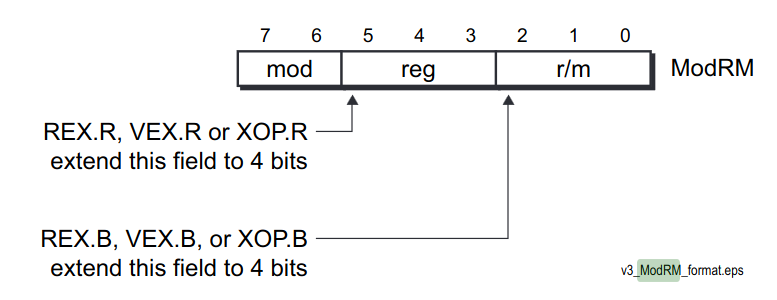
\includegraphics[scale=0.3]{images/img1.png}
		\caption{فرمت بایت ModRM}
		\label{فرمت بایت}
	\end{figure}
\end{center}

حال پس از آشنایی با تفاوت عملکرد opcode ها، D8h و DCh مبدا و مقصد عمگرهای تفریق و محل ذخیره را تعیین می‌کنند.

به مسیر \texttt{src/arch/x86/isa/decoder/x87.isa} می‌رویم و در فایل \texttt{x87.isa} جملات \texttt{FSUBR} را به \texttt{Inst::FSUBR1(Ed)} و \texttt{Inst::FSUBR2(Eq)} و  \texttt{Inst::FSUBR2(Mq)} تغییر می‌دهیم.

سپس به مسیر \texttt{src/arch/x86/isa/insts/x87/arithmetic} می‌رویم و در فایل \texttt{subtraction.py} پیاده‌سازی \texttt{macro-op} ها را انجام می‌دهیم. این پیاده سازی ها باید متنانسب و به تعداد توابع \texttt{FSUB} به کار رفته در این فایل انجام شود. 

\texttt{Macro-op} های نوشته شده برای عملیات \texttt{FSUBR} به صورت زیر است:
\begin{latin}
	\lstinputlisting[
	label={lst:FSUBR_MicroOp},
	language=python,
	style=myStyle,
	]{codes/FSUBR_MicroOp.py}
\end{latin}

در \texttt{macro-op} های بالا در خط \texttt{subfp} عملگر اول رجیستر محل ذخیره سازی خروجی است و دو عملگر بعدی رجیستر هایی هستند که قرار است با هم تفریق شوند.

برای پیاده‌سازی \texttt{subfp micro-op} نیازی نیست کاری انجام دهیم چرا که این پیاده سازی در فایل \texttt{fpop.isa} در مسیر \texttt{src/arch/x86/isa/micro-ops/} وجود دارد.

سپس با دستور \texttt{scons build/X86/gem5.opt -j 9} جم‌۵ را برای معماری \texttt{x86} کامپایل می‌کنیم تا مطمئن شویم در پیاده سازی اشتباهی رخ نداده است.

با اجرای دستور گفته شده خروجی زیر حاصل می‌شود که نشان‌دهنده آن است در مراحل پیاده‌سازی دچار مشکل نشده ایم و پیاده‌سازی با موفقیت انجام شده است.
\begin{center}
	\begin{figure}[H]
		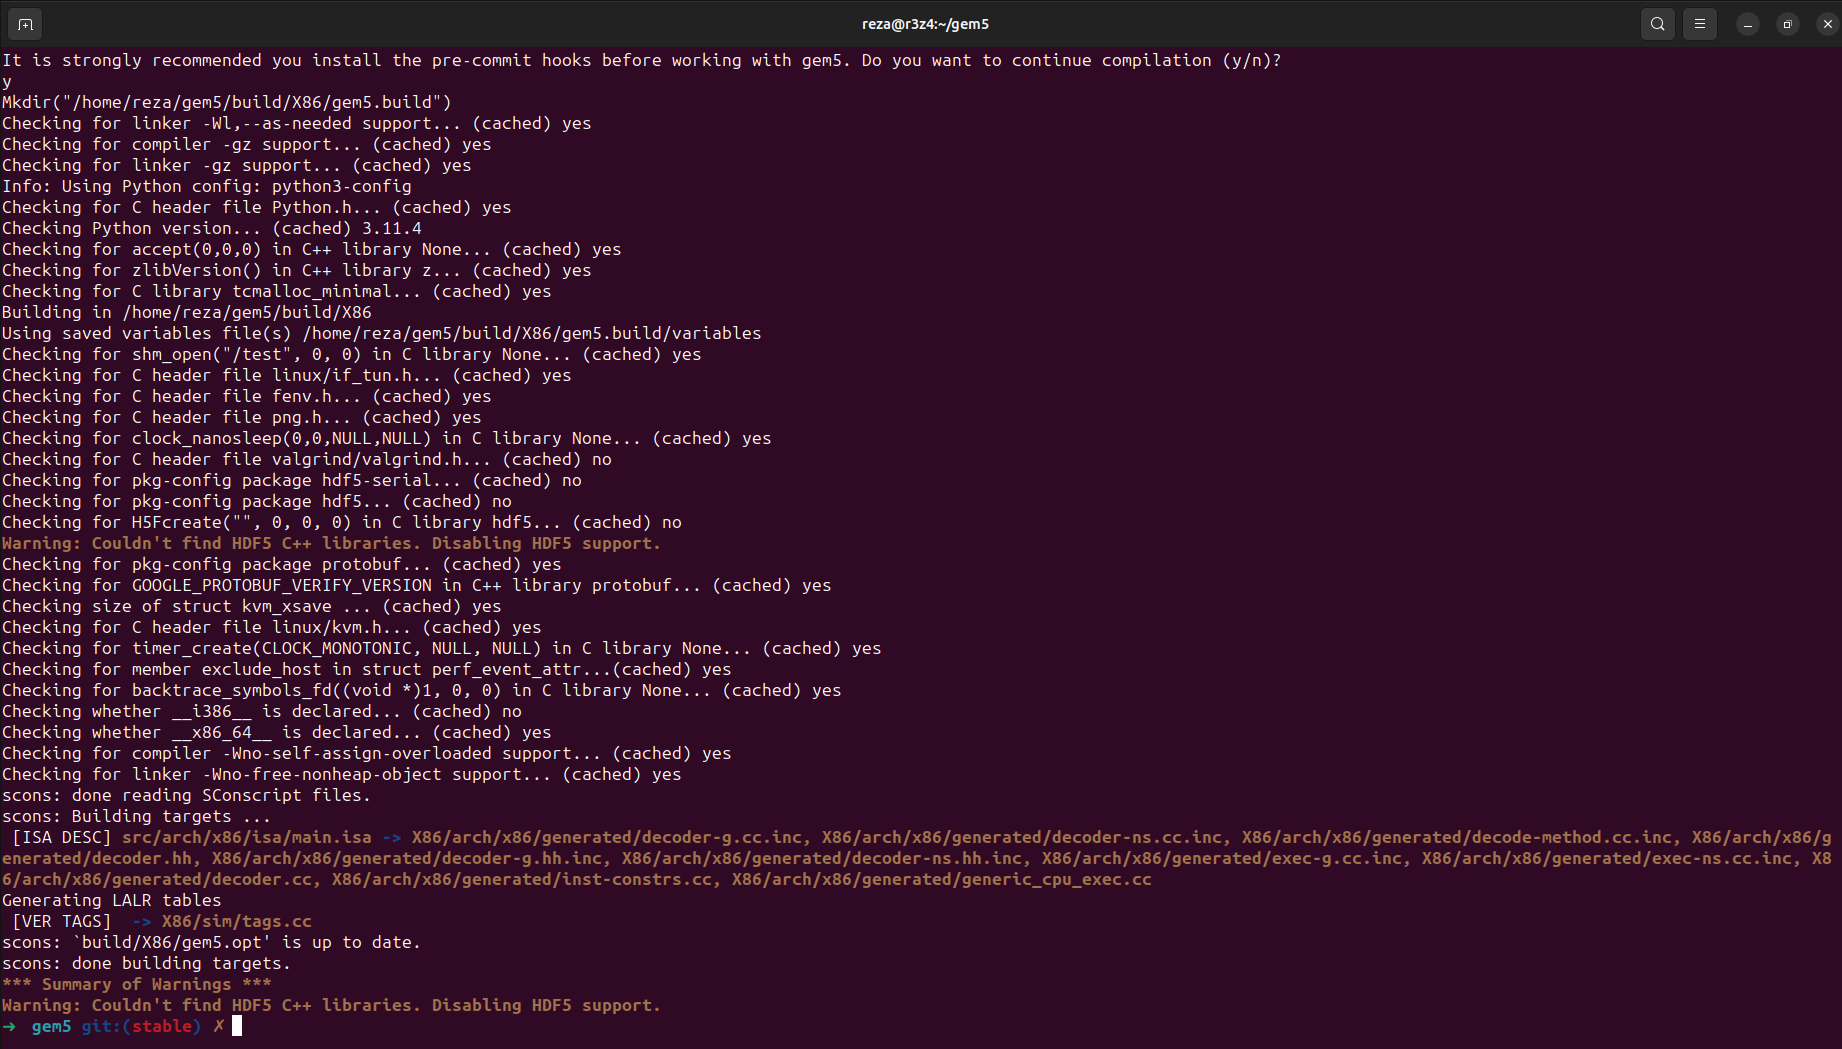
\includegraphics[scale=0.13]{images/img2.png}
		\caption{کامپایل مجدد Gem5}
		\label{کامپایل جم‌۵}
	\end{figure}
\end{center}

و در مرحله اخر برای تست دستور \texttt{FSUBR} برنامه ای به زبان \texttt{C} نوشتیم که از فایل \texttt{random\_numbers.txt} دو عدد را بخواند و عملیات \texttt{FSUBR} را انجام دهد. دو عدد خوانده شده از فایل به صورت رندوم تولید می‌شود. کد نوشته شده در \textbf{«پیوست آ»} آورده شده است.

با کامپایلر gcc کد نوشته شده را build و اجرا می‌کنیم می‌کنیم:
\begin{center}
	\begin{figure}[H]
		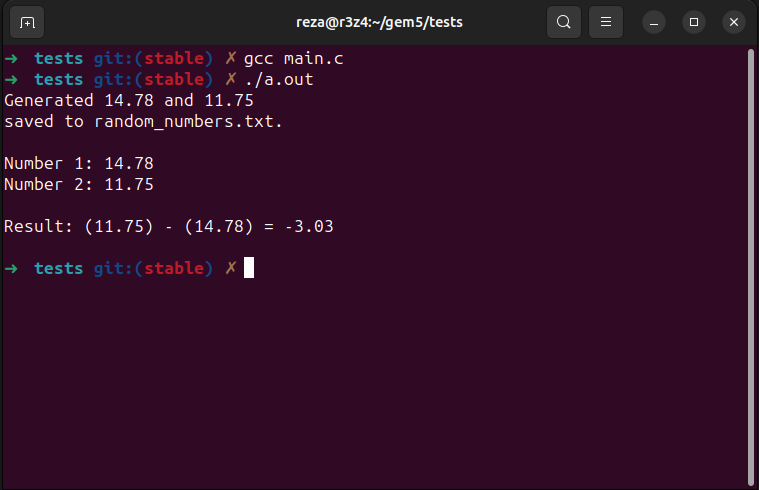
\includegraphics[scale=0.31]{images/img3.png}
		\caption{کامپایل برنامه نوشته شده}
		\label{کامپایل کد}
	\end{figure}
\end{center}

سپس خروجی \texttt{a.out} تولید شده را با دستور زیر در محیط جم‌۵ اجرا می‌کنیم:

\begin{latin}
	\texttt{build/X86/gem5.opt configs/deprecated/}
	\texttt{example/se.py --cmd=tests/a.out}
\end{latin} 

خروجی شبیه سازی به درستی اجرا شده است و ورودی دوم را منهای ورودی اول کرده است:

\begin{center}
	\begin{figure}[H]
		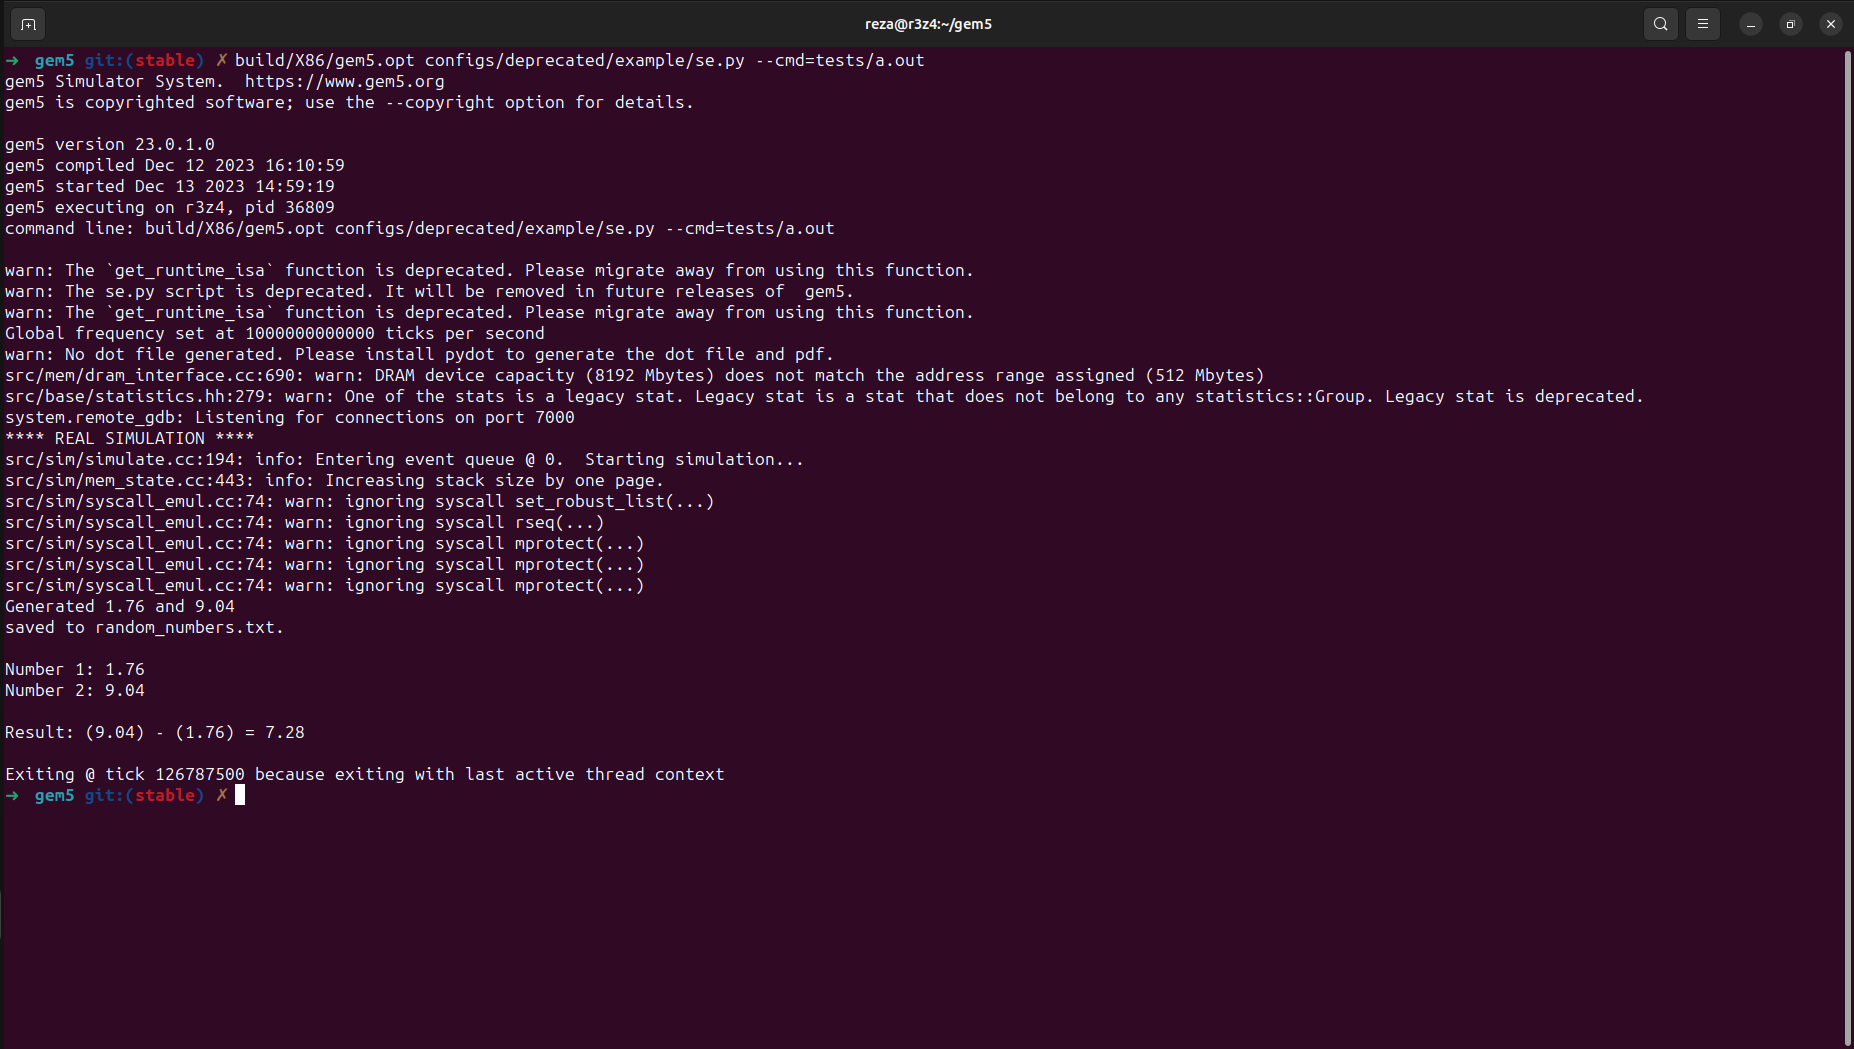
\includegraphics[scale=0.13]{images/img4.png}
		\caption{خروجی شبیه‌سازی}
		\label{شبیه‌سازی در جم}
	\end{figure}
\end{center}


در نهایت با دستور \texttt{git diff src/arch/x86/isa > /tmp/changes.patch} از تغییراتی که در فایل ها انجام دادیم، یک log می‌گیریم.

\begin{center}
	\begin{figure}[H]
		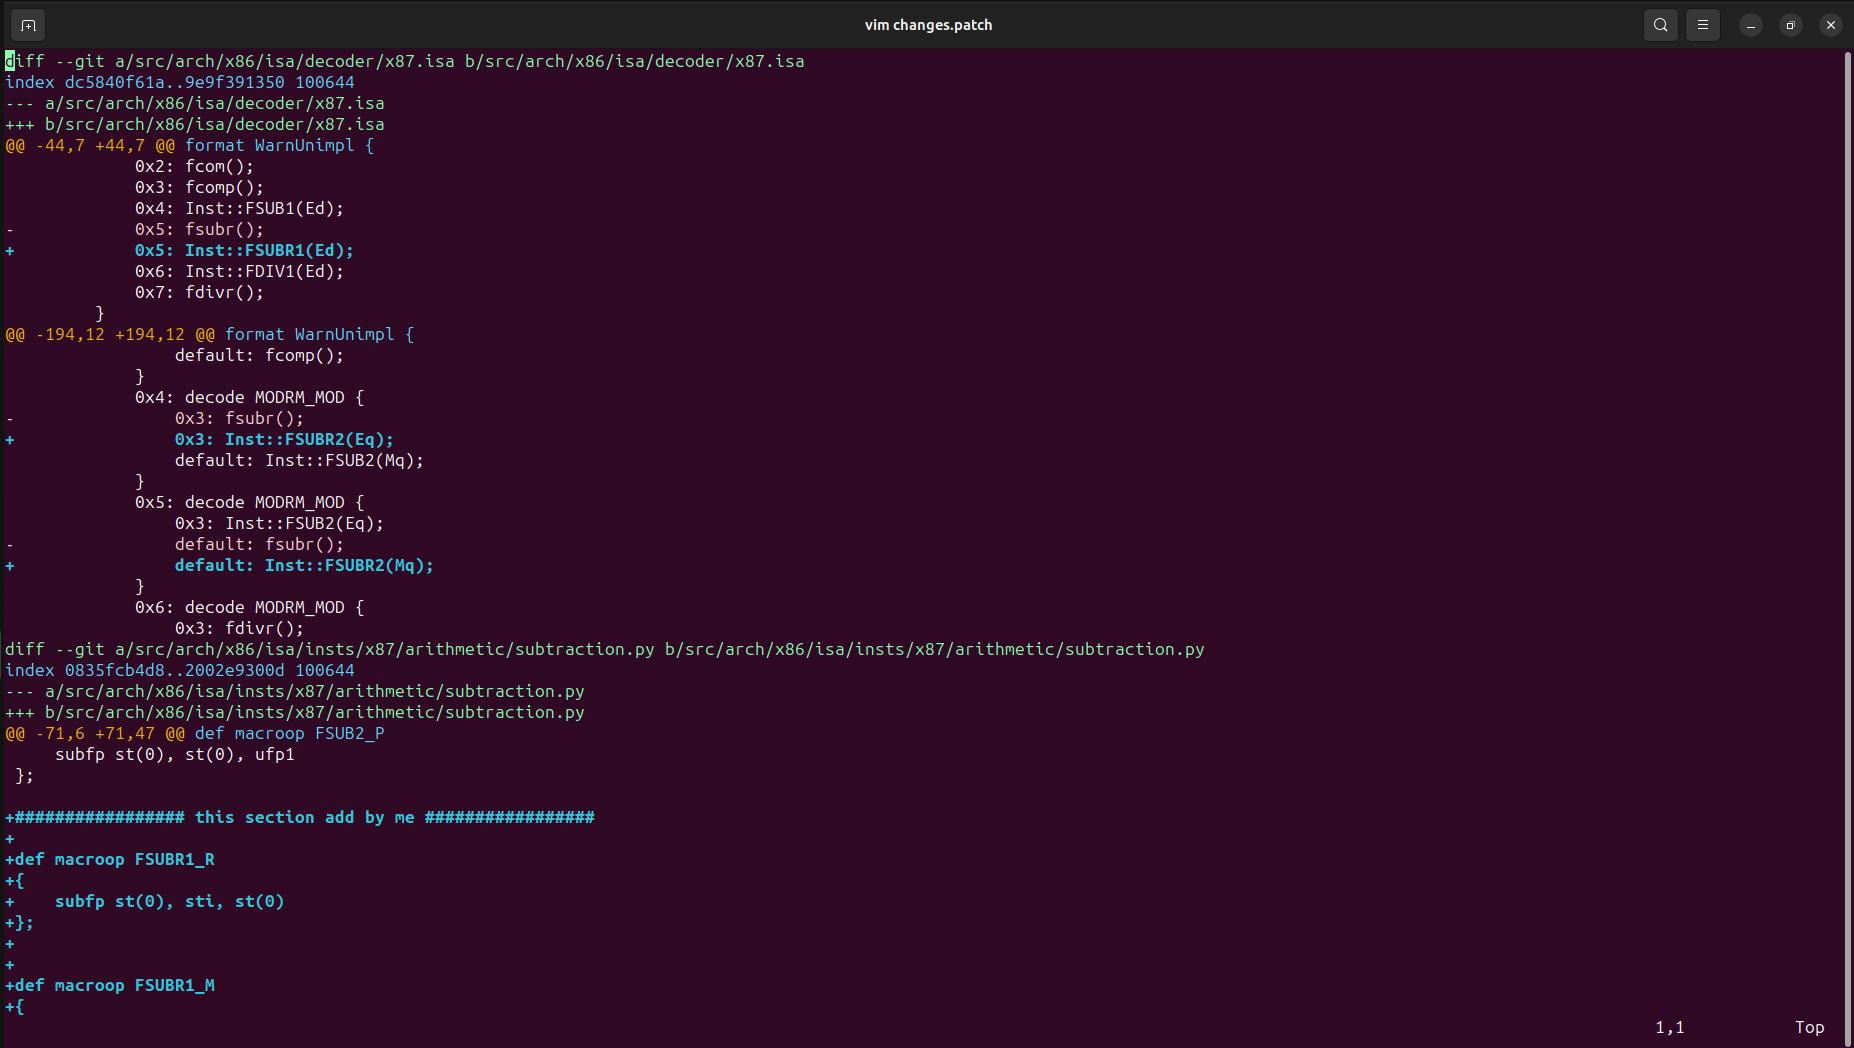
\includegraphics[scale=0.13]{images/img5.png}
		\caption{هیستوری تغییرات}
		\label{هیستوری تغییرات}
	\end{figure}
\end{center}




	
	
\end{multicols}












\newpage
\fontsize{30}{30} \textbf{پیوست آ\label{پیوست آ}} \\ \\ \\


• کد C نوشته شده برای تست FSUBR: 
\begin{latin}
	\lstinputlisting[
	caption=C++ code for part1,
	label={lst:listing-cpp},
	language=C++,
	style=myStyle,
	]{codes/main.c}
\end{latin}

\end{document}